\chapter{Katakana Training - 片仮名練習}\label{chap:KatakanaTraining}

\normalsize

Every person is learning in a different way. What works well for one does not
need to work well also for the other. Because of this an ultimate receipt to
learn Katakana can not be given here. However the introduction to this chapter
would like to try to give some  hints gathered from learning and teaching
experience. 

\begin{description}

\item[Not too less:] If one learns one character per day, it will take for
Katakana roughly 46 days.  If you restrict this to working days it will take
approximately two month. If you restrict it to a 2h lesson per week it will
take a year to learn Katakana. It is obvious that one is likely to forget the
first characters when learning the last. However, even with this method it is
not impossible, but not likely.

\item[Not too much:]  To learn Katakana in one day is unlikely possible. At
least parts will be forgotten the next day.

\end{description}

From the practice the best results have been seen when learners have tried to
learn Katkana in one to three weeks. The suggestion is to learn one line (five
characters) per day in a cumulative way. Means, repeat every day the already
learned characters and that up to 10 days until all are learned. And then
repeat this exercise until they hardly can not be forgotten any more. So for
at least 14 consecutive days without break. 

\begin{description}

\item[Develop your own style:] Learning one character at a time or a row (five
characters at a time) or learn the whole table of Katakana is possible. With
some method it can take 3 weeks or with an other method 1 week. That does not
matter. What do matter is that oneself is comfortable with the method and that
oneself extract fun out of it, even when forced to learn Katakana. Decide by
yourself how often you repeat. But decide. And write down your decision. Maybe
even plan it in your daily plan. A good practice is to learn Katakana 20 times
a day for five minutes rather then one time for three hours a day or one time a
week for 10 hours. 

\item[Search for aid:] Aid can come in may manifestations. Of course it is
useful to ask a Japanese to help. But there are many other ways for helping
yourself.  One example are flashcards. Of course it is easy to print them in
this book. However as said before: find your own way. And if you create
flashcards by yourself you already learn the content up to a certain level. 

\item[Use Squares:] Some European languages uses lines to teach letters. In
Japanese you should use a square and draw the letter in the middle. If
uncertain about the shape and orientation of the character use a square and
look at the squares filled with Katakana in this section to understand the
alignment and orientation.

\end{description}

\newpage

Here are some examples for flashcards. But feel free to invent your own.


\begin{center}
\begin{tabular}{cc}
\textbf{front site Katakana}&\textbf{back site Romaji}\\
\includegraphics[scale=1.5]{../share/i/fcar.pdf}% Romaji - Katakana
&
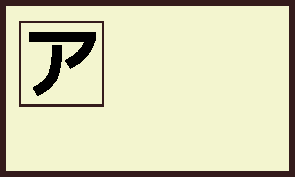
\includegraphics[scale=1.5]{../share/i/fcak.pdf}% Hiragana Katakana
\\
\end{tabular}
\end{center}

Or to learn both:

\begin{center}
\begin{tabular}{cc}
\textbf{front site Romaji}&\textbf{back site both}\\
\includegraphics[scale=1.5]{../share/i/fcar.pdf}% Romaji - Katakana
&
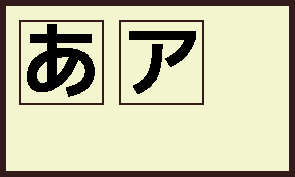
\includegraphics[scale=1.5]{../share/i/fcahk.pdf}% Hiragana Katakana
\\
\end{tabular}
\end{center}

To dive deep into Japanese of course skipping Romaji is the preferred method:

\begin{center}
\begin{tabular}{cc}
\textbf{front site Katakana}&\textbf{back site Hiragana}\\
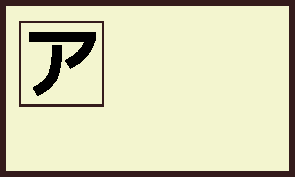
\includegraphics[scale=1.5]{../share/i/fcak.pdf}% Romaji - Katakana
&
\includegraphics[scale=1.5]{../share/i/fcah.pdf}% Hiragana Katakana
\\
\end{tabular}
\end{center}

This training chapter can be used as an additional aid to learn Katakana. And
also here it is important to develop ones own method. However some hints on
learning with this training chapter can be given.

\begin{description}

\item[Reading Loud:] While writing a Katakana character in this book (and
probably also later), read out loud the sound of the character. Always. 

\item[Invent your own cribs:] One can (maybe should?) invent one crib per
character by oneself. Especially if the characters is difficult to remember. It
might be useful to write it down on the self created flashcard for that
specific character.

\item[Regular Repetition:] It is of course possible to fill out all fields
for one chracter in a very short time. The learning effect should be minimal
though. Better is to fill out one row and then the second row an hour later,
the third row the next day and so own. Oneself has to decide the rhythm of
the repetition. 

\item[Transcription:]  Search for a  Katakana text and read it. Write for every
Katakana word the Roman letters. If this is possible without looking up the
Katakana, then the transcription should be reversed. Find some Japanese text
written in Romaji and transcribe them on Katakana on a different piece of
paper. 

\end{description}

\newpage

\section{片仮名 ア行 - Katakana |a| Row}  \label{sec:KatakanaARow}

\Krow{arow}{a}{i}{u}{e}{o}

\label{letter:a}\KLETTER{a} The 片仮名 {「ア」} derives from the
\hyperref[sec:Manyogana]{万葉仮名} characters {「阿」} left element
(\hyperref[sec:Radical]{radical}).  A smaller version {「ァ」} is used in
combinations with other letters as {「ファ」} and is pronounced as |fa| in
\hyperref[sec:Hepburn]{Hepburn} transcription.

\label{letter:u}\KLETTER{i} The 片仮名 {「イ」} derives from the
\hyperref[sec:Manyogana]{万葉仮名} characters {「伊」} left element
(\hyperref[sec:Radical]{radical}).  A smaller version {「ィ」} is used in
combinations with other letters and represents a
\hyperref[sec:Diphthong]{diphthong}. 

\label{letter:u}\KLETTER{u} The 片仮名 {「ウ」} derives from the
\hyperref[sec:Manyogana]{万葉仮名} character {「宇」}. A smaller version
{「ゥ」} is used in combinations with other letters and represents a
\hyperref[sec:Diphthong]{diphthong} and is written as "w". Even though the
combination {「トゥ」} |tu| exist, it is relatively new and many words do not
use it. In this cases {「ツ 」} |tsu| is used. {「ウ」} can take
\hyperref[sec:Dakuten]{Dakuten} to form {「ヴ」} |vu|, which is relatively new
and can replace {「ブ」} |bu|. 

\Note{Note}{%

Be aware that the characters \hyperref[letter:fu]{「フ」},
\hyperref[letter:wa]{「ワ」}  and \hyperref[letter:u]{「ウ」} look very
similar.  Make sure that you spend extra training on distinguish them. 

}%


\newpage 

\label{letter:e}\KLETTER{e} The 片仮名 {「エ」} derives from the
\hyperref[sec:Manyogana]{万葉仮名} characters {「江」} right element
(\hyperref[sec:Radical]{radical}). A smaller version {「ェ」} is used in
combinations with other letters and express \hyperref[sec:Mora]{morae} of
foreign origin. For example {「ヴェ」} as pronounced |ve|.

\label{letter:o}\KLETTER{o} The 片仮名 {「オ」} derives from the
\hyperref[sec:Manyogana]{万葉仮名} character {「於」}. A smaller version
{「ォ」} is used in combinations with other letters and express
\hyperref[sec:Mora]{morae} of foreign origin. For example {「フォ 」} as
pronounced |fe|.

\newpage


% ---------------------------------------------------------------------------
\subsection{ア - |a|} \label{sec:KatakanaA}

\KatakanaHeader{a}{ The Katakana {「ア」} is written with two strokes. The
first stroke starts horizontal. The second stroke is a curve with can be
attached to the first stroke in hand writing, but not at the horizontal part -
at the end of the first line.} \KatakanaTraining{a}

% ---------------------------------------------------------------------------
\subsection{イ - |i|} \label{sec:KatakanaI}

\KatakanaHeader{i}{ The Katakana {「イ」} is written with one stroke. The first
stroke is a curve from upper right to lower left. The second stroke is a
vertical line attached to the first at the top.} \KatakanaTraining{i}

% ---------------------------------------------------------------------------
\subsection{ウ - |u|} \label{sec:KatakanaU}

\KatakanaHeader{u}{The Katakana {「ウ」} is written with three strokes. The
first stroke a small vertical line. The second a small vertical line again and
the third line a horizontal line connection the two others.}
\KatakanaTraining{u}

% ---------------------------------------------------------------------------
\subsection{エ - |e|} \label{sec:KatakanaE}

\KatakanaHeader{e}{The Katakana {「エ」} is written with three strokes. It is
very geometrically consisting only out of horizontal and vertical lines
connected together.} \KatakanaTraining{e}

% ---------------------------------------------------------------------------
\subsection{オ - |o|} \label{sec:KatakanaO}

\KatakanaHeader{o}{The Katakana {「オ」} is written with three strokes. The
first line is horizontal and together with the second stroke it constructs a
perfect crossing. The third stroke beginning lies at the center of the
crossing.} \KatakanaTraining{o}

\section{片仮名ア行練習 -  |a| Row Training}

\KatakanaSimpleTraining{Katakana to Romaji}{
\Transcribe{1.}{ウエア}{}{wear, ware}
\Transcribe{2.}{エア}{}{air}
\Transcribe{3.}{エイ}{}{A (the letter)}
\Transcribe{4.}{アイ}{}{I (the letter)}
\Transcribe{5.}{オウ}{}{O (the letter)}
\Transcribe{6.}{イア}{}{ear}
}

\KatakanaSimpleTraining{Romaji to Katakana}{
\Transcribe{1.}{ea}{}{air}
\Transcribe{2.}{ai}{}{I (the letter)}
\Transcribe{3.}{ou}{}{O (the letter)}
\Transcribe{4.}{ei}{}{A (the letter)}
\Transcribe{5.}{uea}{}{wear, ware}
\Transcribe{6.}{ia}{}{ear}
}

\newpage

\KatakanaSimpleTraining{English to Romaji}{
\Transcribe{1.}{ear}{}{}
\Transcribe{2.}{I (the letter)}{}{}
\Transcribe{3.}{air}{}{}
\Transcribe{4.}{O (the letter)}{}{}
\Transcribe{5.}{wear, ware}{}{}
\Transcribe{6.}{A (the letter)}{}{}
}

\KatakanaSimpleTraining{English to Katakana}{
\Transcribe{2.}{I (the letter)}{}{}
\Transcribe{3.}{O (the letter)}{}{}
\Transcribe{1.}{air}{}{}
\Transcribe{6.}{ear}{}{}
\Transcribe{5.}{wear, ware}{}{}
\Transcribe{4.}{A (the letter)}{}{}
}
\newpage
   % OK
% ---------------------------------------------------------------------------
\section{Katakana /ka/ Row}\jsec{片仮名 カ行}\label{sec:KatakanaKaRow}

\Krow{karow}{ka}{ki}{ku}{ke}{ko}

\label{letter:ka}\KLETTER{ka} The  片仮名 {「カ」} is pronounced  /ka/ and  derives from the
\hyperref[sec:PhoneticCharacter]{Phonetic Character}s {「加」} left
\hyperref[sec:Radical]{radical}.  A \hyperref[sec:Dakuten]{濁点} version exists
and pronounced as /ga/.

%\hyperref[sec:Handakuten]{半濁点} does not exist in daily Japanese.  
% {「一ヵ所」} {【いちかしょ】} (one place)
% {「一ヶ所」} {【いちかしょ】} (one place).
% 十ヵ条(十ヶ条)


\Note{Note}{A smaller version {「ヵ」} is rare but used in combinations with
number particles.  For example in {「一ヵ月」} {【いっかげつ】} (one month) and
others.  This cases can also be written {「一ヶ月」} {【いっかげつ】} (one
month). Please see also \nameref{sec:KatakanaKe}. \Link
\href{http://ja.wikipedia.org/wiki/\%E3\%83\%B5}{ヵ} }

\label{letter:ki}\KLETTER{ki} The 片仮名 {「キ」} derives from the
\hyperref[sec:PhoneticCharacter]{Phonetic Character}s middle part of either {「機」} or
{「幾」}.  It is pronounced as /ki/.  A \hyperref[sec:Dakuten]{濁点} version
exists and pronounced as /gi/.


\label{letter:ku}\KLETTER{ku} The 片仮名 {「ク」} derives from the
\hyperref[sec:PhoneticCharacter]{Phonetic Character}s left upper part of {「久」}.  It
is pronounced as /ku/.  A \hyperref[sec:Dakuten]{濁点} version exists and
pronounced as /gu/.  A smaller version exists, but is used for the Ainu
Language.



\label{letter:ke}\KLETTER{ke} The 片仮名 {「ケ」} derives from the
\hyperref[sec:PhoneticCharacter]{Phonetic Character}s upper and left part of {「介」}.
It is pronounced as /ke/.  A \hyperref[sec:Dakuten]{濁点} version exists and
pronounced as /ge/.  The smaller version {「ヶ」} is explained in the following
note.

\newpage

\Note{Note}{ A smaller version {「ヶ」} is rare but used in combinations with
number particles.  For example in {「一ヶ月」} {【いっかげつ】} (one month) and
others.  This cases can also be written {「一ヵ月」} {【いっかげつ】} (one
month). There are cases where only {「ヶ」} can be written {七ヶ宿}
{【シチカシュク】} (Place at the south west border of the prefecture Miyagi).
In other rare cases this character can be pronounced different {「関ヶ原」}
{【せきがはら】} (Place at the south border of the Gifu prefecture, known by
the battle at 1600.). Please see also \nameref{sec:KatakanaKa}. \Link
\href{http://ja.wikipedia.org/wiki/\%E3\%83\%B5}{ヵ} }

\label{letter:ko}\KLETTER{ko} The 片仮名 {「コ」} derives from the
\hyperref[sec:PhoneticCharacter]{Phonetic Character}s upper part of {「己」}.  It is
pronounced as /ko/.  A \hyperref[sec:Dakuten]{濁点} version exists and
pronounced as /go/.



\newpage

% ---------------------------------------------------------------------------
\subsection{/ka/}\jsubsec{「カ」} \label{sec:KatakanaKa}

\KatakanaHeader{ka}{ /ka/ is written with 2 strokes. Basically the same way as
the Hiragana {「か」} it looks like a squarish version, but without the last
stroke. The hook at the second stroke is less significant or important.  }
\KatakanaTraining{ka}

% ---------------------------------------------------------------------------
\subsection{/ki/}\jsubsec{「キ」} \label{sec:KatakanaKi}

\KatakanaHeader{ki}{ The shape alignment of the 「キ」character is not straight
towards its environment. However the junctions are more or less 90 degrees.  }
\KatakanaTraining{ki}

% ---------------------------------------------------------------------------
\subsection{/ku/}\jsubsec{「ク」} \label{sec:KatakanaKu}
% ---------------------------------------------------------------------------

\KatakanaHeader{ku}{ The first stroke is similar the stroke of {「ケ 」} is a
curve. While the second stroke start aligned and straight. }
\KatakanaTraining{ku}

% ---------------------------------------------------------------------------
\subsection{/ke/}\jsubsec{「ケ」} \label{sec:KatakanaKe}

\KatakanaHeader{ke}{ The {「ケ 」} is written with 3 strokes and the first
stroke is similar to the {「ク」}. The second stroke is aligned and straight.
While the last stroke is a curve.  } \KatakanaTraining{ke}

% ---------------------------------------------------------------------------
\subsection{/ko/}\jsubsec{「コ」} \label{sec:KatakanaKo}

\KatakanaHeader{ko}{ This character is almost a geometric figure composed out
of two strokes. However unless in European languages this are only 2 strokes
and not 3. The first stroke is the longest one and done similar with all
{漢字}. } \KatakanaTraining{ko}

% ---------------------------------------------------------------------------
\subsection{/ka/ Row Training}\jsubsec{片仮名カ行練習}

\Padding
\begin{longtable}[c]{p{2cm}p{1.5cm}p{1.5cm}p{3cm}p{7cm}}
\textit{Katakana}&\textit{Rōmaji}&\textit{Original}&\textit{Remark}&Origin\\\hline
カキ  &kaki &kaki &柿 persimon&Japanese\\
ケア  &kea  &care &          &English\\
ケイ  &kei  &K    &the letter&English\\
\end{longtable}

\KatakanaSimpleTraining{Katakana to Rōmaji}{
\Transcribe{1.}{カキ}{}{persimmon}
\Transcribe{2.}{ココア}{}{cocoa}
\Transcribe{3.}{ケア}{}{care}
\Transcribe{4.}{コア}{}{core}
\Transcribe{5.}{ケーキ}{}{cake}
%\Transcribe{6.}{ケイ}{}{K (the letter)}
}

\KatakanaSimpleTraining{Rōmaji to Katakana}{
\Transcribe{1.}{kokoa}{}{cocoa}
\Transcribe{2.}{k$\overline{\mbox{e}}$ki}{}{cake}
\Transcribe{3.}{kea}{}{care}
\Transcribe{4.}{koa}{}{core}
\Transcribe{5.}{kaki}{}{persimmon}
%\Transcribe{6.}{kei}{}{K (the letter)}
}

\newpage

\Padding
%\begin{longtable}[c]{p{2cm}p{2cm}p{3cm}p{6cm}p{2cm}}
\begin{longtable}[c]{p{2cm}p{2.0cm}p{3.5cm}p{4cm}p{2.5cm}}
\textit{Katakana}&\textit{Rōmaji}&\textit{Original}&\textit{Remark}&Origin\\\hline
コア  &koa  &core &          &English\\
ココア&kokoa&cocoa& hot chocolate &English, from metathesis of Spanish cacao, from Nahuatl cacahuatl\\
ケーキ&kēki &cake &          &English\\
\end{longtable}


\KatakanaSimpleTraining{English to Rōmaji}{
\Transcribe{1.}{persimon}{}{}
\Transcribe{2.}{cocoa}{}{}
\Transcribe{3.}{care}{}{}
\Transcribe{4.}{core}{}{}
\Transcribe{5.}{K (the letter)}{}{}
%\Transcribe{6.}{cake}{}{}
}

\KatakanaSimpleTraining{English to Katakana}{
\Transcribe{1.}{cocoa}{}{}
\Transcribe{2.}{cake}{}{}
\Transcribe{3.}{care}{}{}
\Transcribe{4.}{persimon}{}{}
\Transcribe{5.}{K (the letter)}{}{}
%\Transcribe{6.}{core}{}{}
}

\newpage
  % OK
\section{片仮名  サ行 - Katakana |sa| Row} \label{sec:KatakanaSaRow}

\Krow{sarow}{sa}{shi}{su}{se}{so}

\KLETTER{sa} The  片仮名 {「サ」} is pronounced  |sa| and  derives from the
\hyperref[sec:Manyogana]{万葉仮名} characters {「散」} upper left corner
\hyperref[sec:Radical]{radical}.  A \hyperref[sec:Dakuten]{濁点} version exists
and pronounced as |za|.

\KLETTER{shi} The 片仮名 {「シ」} derives from the
\hyperref[sec:Manyogana]{万葉仮名} character  {「之 」}.  It is pronounced as
|shi|.  A \hyperref[sec:Dakuten]{濁点} version exists and pronounced as |ji|.

\Note{Note}{Please see section \nameref{subsec:ShiTsuAmbiguity} for the
explanation how to write and distinguish |shi| and |tsu|.  }

\KLETTER{su} The 片仮名 {「ス」} derives from the
\hyperref[sec:Manyogana]{万葉仮名} characters right lower part of {「須」}.  It
is pronounced as |su|.  A \hyperref[sec:Dakuten]{濁点} version exists and
pronounced as |zu|. 

\KLETTER{se} The 片仮名 {「セ」} derives from the
\hyperref[sec:Manyogana]{万葉仮名} characters middle left part of {「世」}.
It is pronounced as |se|.  A \hyperref[sec:Dakuten]{濁点} version exists and
pronounced as |ze|.  

\newpage

\KLETTER{so} The 片仮名 {「ソ」} derives from the
\hyperref[sec:Manyogana]{万葉仮名} characters upper right part of {「曽」}.  It is
pronounced as |so|.  A \hyperref[sec:Dakuten]{濁点} version exists and
pronounced as |zo|.

% SoRiNAmbiguity
\subsection{|so|, |ri| and |n| Ambiguity} \label{subsec:SoRiNAmbiguity}

The Katakana characters {「ソ」}, {「リ」} and {「ン」} can be difficult to
distinguish. All three are made out of only 2 strokes. And especially |so| and
|n| can be hard to tell. In a sentence of course the context can help a lot.
But what are the rules for this characters to write properly and distinguish?

\bigskip

\begin{center}
\begin{tabular}{|c|c|c|}\hline
\KLETTER{so}&\KLETTER{n}&\KLETTER{ri}\\\hline
\end{tabular}
\end{center}

\CharacterExplanation{soexplanation}{ To write the letter |so| it is important
to align both lines \textbf{horizontally} (red line) and to \textbf{non-align}
the ends (blue line).  In this way it is possible to distinguish |so| from |n|,
but not from |ri|. To also distinguish it from |ri| you have to write the first
stroke not horizontally nor vertically.  }

\CharacterExplanation{nexplanation}{ To write the letter |n| it is important to
a align both lines \textbf{vertically} (red line) and to \textbf{non-align} the
ends (blue line). In this way it is possible to distinguish |n| from |so|. If
both lines are aligned there should not be a problem to distinguish it from
|ri|.  }

\CharacterExplanation{riexplanation}{ To write the letter |ri| it is important
to a align both lines \textbf{vertically} (red line) and to \textbf{non-align}
the ends (blue line). The difference between |so| and |ri| is that |ri| need to
start with two \textbf{parallel} lines wile |so| does not. Please see green
lines for explanation.  }




\newpage

\subsection{サ - |sa|} \label{sec:KatakanaSa}

\KatakanaHeader{sa}{ Katakana {「サ」} is written with three strokes. All
crossings of strokes are in a 90 degree angle.  The starts of all strokes are
aligned eitehr horizontally or vertically. The last stroke has a curve.}
\KatakanaTraining{sa}

\subsection{シ - |shi|} \label{sec:KatakanaShi}

\KatakanaHeader{shi}{ The Katakana {「シ」} is written with three strokes. All
three strokes are aligned vertically in the beginning. Please see section
\nameref{subsec:ShiTsuAmbiguity}.}

\KatakanaTraining{shi}

\subsection{ス - |su|} \label{sec:KatakanaSu}

\KatakanaHeader{su}{The Katakana {「ス」} is written with two strokes. The first
stroke startes horizontally aligned. The second stroke touches the first stroke
at the beginning.}

\KatakanaTraining{su}

\subsection{セ - |se|} \label{sec:KatakanaSe}

\KatakanaHeader{se}{ The Katakana {「セ」} is written with two strokes. The
crossing has \textbf{no} 90 degree angle. The curve of the second stroke as
almost a 90 deegre angle. } 

\KatakanaTraining{se}

\subsection{ソ - |so|} \label{sec:KatakanaSo}

\KatakanaHeader{so}{ The Katakana {「ソ」} is written with two strokes. The
first stroke is not aligned verticall but it is aligned horizontally withe the
second stroke. Please see section \nameref{subsec:SoRiNAmbiguity}.}

\KatakanaTraining{so}

\section{片仮名サ行練習 -  |sa| Row Training}
% 3 78 エキス 
%3 357 スカイ 
%3 360 スキー 
%3 3 アイス 
%3 111 ガーゼ 
%3 146 イエス
\renewcommand*{\arraystretch}{1.4}
\begin{longtable}[c]{p{2cm}p{2cm}p{3cm}p{6cm}p{2cm}}
エキス&ekisu&ex(tract)&extract&Dutch\\
スカイ&sukai&sky&&English\\
スキー&sukī&ski&noun for skiing&English\\
\end{longtable}
\KatakanaSimpleTraining{Katakana to Romaji}{
\Transcribe{1.}{エキス}{}{extract}      % ekisu
\Transcribe{2.}{スカイ}{}{sky}          % sukai
\Transcribe{3.}{スキー}{}{ski}          % sukī
\Transcribe{4.}{アイス}{}{ice}          % aisu
\Transcribe{5.}{ガーゼ}{}{gauze}        % gāze
\Transcribe{6.}{イエス}{}{Jesus}        % iesu
}

\KatakanaSimpleTraining{Romaji to Katakana}{
\Transcribe{1.}{sukai}{}{sky}         % sukai
\Transcribe{2.}{ekisu}{}{extract}     % ekisu
\Transcribe{3.}{aisu}{}{ice}          % aisu
\Transcribe{4.}{suki}{}{ski}          % sukī
\Transcribe{5.}{iesu}{}{Jesus}        % iesu
\Transcribe{6.}{gāze}{}{gauze}        % gāze
}

\newpage
\renewcommand*{\arraystretch}{1.4}
\begin{longtable}[c]{p{2cm}p{2cm}p{3cm}p{6cm}p{2cm}}
\textit{Katakana}&\textit{Rōmaji}&\textit{Original}&\textit{Remark}&Origin\\\hline
アイス&aisu&ice&water ice, ice cream&English\\
ガーゼ&gāze&Gaze&gauze&German\\
イエス&iesu&Jesus&Jesus&Portuguese\\
\end{longtable}
\KatakanaSimpleTraining{English to Romaji}{
\Transcribe{1.}{extract}{}{}       % ekisu
\Transcribe{2.}{sky}{}{}           % sukai
\Transcribe{3.}{Jesus}{}{}         % iesu
\Transcribe{4.}{gauze}{}{}         % gāze
\Transcribe{5.}{ice}{}{}           % aisu
\Transcribe{6.}{ski}{}{}           % sukī
}

\KatakanaSimpleTraining{English to Katakana}{
\Transcribe{1.}{sky}{}{}           % sukai
\Transcribe{2.}{gauze}{}{}         % gāze
\Transcribe{3.}{ice}{}{}           % aisu
\Transcribe{4.}{Jesus}{}{}         % iesu
\Transcribe{5.}{extract}{}{}       % ekisu
\Transcribe{6.}{ski}{}{}           % sukī
}

\newpage
  % OK
% タチツテト
\section{片仮名  タ行 - Katakana |ta| Row}  \label{sec:KatakanaTaRow}

\Krow{tarow}{ta}{chi}{tsu}{te}{to}

\KLETTER{ta} The  片仮名 {「タ」} is pronounced  |ta| and  derives from the
\hyperref[sec:Manyogana]{万葉仮名} characters {「多 」} upper or lover
\hyperref[sec:Radical]{radical}.  A \hyperref[sec:Dakuten]{濁点} version exists
and pronounced as |da|.

\KLETTER{chi} The 片仮名 {「チ」} derives from the
\hyperref[sec:Manyogana]{万葉仮名} character  {「千」}.  It is pronounced as
|chi|.  A \hyperref[sec:Dakuten]{濁点} version exists and pronounced as |ji|.

\KLETTER{tsu} The 片仮名 {「ツ」} derives from the
\hyperref[sec:Manyogana]{万葉仮名} characters {「州」} or {「川」} .  It is
pronounced as |tsu|.  A \hyperref[sec:Dakuten]{濁点} version exists and
pronounced as |zu|. 

\KLETTER{te} The 片仮名 {「テ」} derives from the
\hyperref[sec:Manyogana]{万葉仮名} characters lower left part of {「天 」}.  It
is pronounced as |te|.  A \hyperref[sec:Dakuten]{濁点} version exists and
pronounced as |de|.  

\newpage

\KLETTER{to} The 片仮名 {「ト」} derives from the
\hyperref[sec:Manyogana]{万葉仮名} characters right part of {「止」}.  It is
pronounced as |to|.  A \hyperref[sec:Dakuten]{濁点} version exists and
pronounced as |do|.

% ShiTsuAmbiguity
\subsection{\jtl{shi} and \jtl{tsu} Ambiguity} \label{subsec:ShiTsuAmbiguity}

% シ
% ツ

The Katakana characters \jquotesingleja{シ} and \jquotesingleja{ツ} are
difficult to distinguish.  Both are made out of 3 strokes and even the length
are equal. In a sentence of course the context can help a lot. But what are the
rules for this characters to write properly and distinguish?

\bigskip

\begin{figure}[H]
\begin{center}
\begin{tabular}{|c|c|}\hline
\KLETTER{shi}&\KLETTER{tsu}\\\hline
\end{tabular}
\end{center}
\caption{\jtl{shi} and \jtl{tsu} ambiguity}
\label{fig:ShiAndTsuAmbiguity}
\end{figure}

\CharacterExplanation{shiexplanation}{

To write the letter \jtl{shi} it is important to align three lines
\textbf{vertically} (red line) and to \textbf{non-align} the ends (blue line).
In this way it is possible to distinguish \jtl{shi} from \jtl{tsu}. Of course
also the angle of the frist two lines are different, but in hadwriting this is
difficult to match. As a rule of thumb make the third line double as long as
the first two but short enough to not align it at the end.

}

\CharacterExplanation{tsuexplanation}{

To write the letter \jtl{tsu} it is important to align all tree lines
\textbf{horizontally} (red line) and to \textbf{non-align} the ends (blue
line). In this way it is possible to distinguish \jtl{tsu} from \jtl{shi}. Of
course also the angle of the first two lines are different, but in handwriting
this is difficult to match. As a rule of thumb make the third line double as
long as the first two but short enough to not align it at the end.

}

 


\newpage

% タチツテト
\subsection{タ - |ta|} \label{sec:KatakanaTa}

\KatakanaHeader{ta}{ Katakana |ta| is written with three strokes. The first
stroke is a small curve. The secosnd stroke starts horizontally attached to the
first stroke. The third stroke ends at the second stroke.}
\KatakanaTraining{ta}

\subsection{チ - |chi|} \label{sec:KatakanaChi}

\KatakanaHeader{chi}{ Katakana |chi| is written with three strokes. The first
stroke is a light curve. The second ihorizontally straight line. The third line
is a curve that joints the first and the second.} \KatakanaTraining{chi}

\subsection{ツ - |tsu|} \label{sec:KatakanaTsu}

\KatakanaHeader{tsu}{Katakana |tsu| is written with three strokes. The first
and second stroke are short. And the beginning of all three strokes is aligned
horizontally. The third stroke is the longest, but the end is not alignd wit
the beginning of the first stroke. } \KatakanaTraining{tsu}

\subsection{テ - |te|} \label{sec:KatakanaTe}

\KatakanaHeader{te}{ Katakana |te| is written with three strokes. The first
stroke is the shortest and horizontally. The second stroke is not aligned
vertically in the beginning, but also perfectly horizontally. The third stroke
is a small curve attached to the middle of the second stroke. }
\KatakanaTraining{te}

\subsection{ト - |to|} \label{sec:KatakanaTo}

\KatakanaHeader{to}{ Katakana |to| is written with 2 strokes. The first stroke
is a vertical line. Attached to this line there is short straight line to the
right. In some hand writings this line is a small curve to the right.}
\KatakanaTraining{to}

\section{片仮名タ行練習 - |ta| Row Training}

\KatakanaSimpleTraining{Katakana to Romaji}{
\Transcribe{1.}{ココア}{}{cocoa}
}

\KatakanaSimpleTraining{Romaji to Katakana}{
\Transcribe{1.}{kokoa}{}{cocoa}
}

\newpage
\KatakanaSimpleTraining{English to Romaji}{
\Transcribe{1.}{persimon}{}{}
}

\KatakanaSimpleTraining{English to Katakana}{
\Transcribe{1.}{cocoa}{}{}
}

\newpage
  % OK
% ナニヌネノ
\section{片仮名  ナ行 - Katakana |na| Row} \label{sec:KatakanaNaRow}

\Krow{narow}{na}{ni}{nu}{ne}{no}

\KLETTER{na} The  片仮名 {「ナ」} is pronounced  |na| and  derives from the
\hyperref[sec:Manyogana]{万葉仮名} characters {「奈」} upper left corner part.
A \hyperref[sec:Dakuten]{濁点} version  or \hyperref[sec:Handakuten]{半濁点} do
not exist.

\KLETTER{ni} The  片仮名 {「ニ」} is pronounced  |ni| and  derives from the
\hyperref[sec:Manyogana]{万葉仮名} characters {「奈」} upper right part.
A \hyperref[sec:Dakuten]{濁点} version  or \hyperref[sec:Handakuten]{半濁点} do
not exist.

\KLETTER{nu} The  片仮名 {「ヌ」} is pronounced  |nu| and  derives from the
\hyperref[sec:Manyogana]{万葉仮名} characters {「奴」} right part.
A \hyperref[sec:Dakuten]{濁点} version  or \hyperref[sec:Handakuten]{半濁点} do
not exist.

\newpage

\KLETTER{ne} The  片仮名 {「ヌ」} is pronounced  |ne| and  derives from the
\hyperref[sec:Manyogana]{万葉仮名} characters {「祢」} upper left  part.
A \hyperref[sec:Dakuten]{濁点} version  or \hyperref[sec:Handakuten]{半濁点} do
not exist.

\KLETTER{no} The  片仮名 {「ノ」} is pronounced  |no| and  derives from the
\hyperref[sec:Manyogana]{万葉仮名} characters {「乃」} upper left part.
A \hyperref[sec:Dakuten]{濁点} version  or \hyperref[sec:Handakuten]{半濁点} do
not exist.
\newpage

% ナニヌネノ
\subsection{ナ - |na|} \label{sec:KatakanaNa}

\KatakanaHeader{na}{ Katakana |na| is written with two strokes.} \KatakanaTraining{na}

\subsection{ニ - |ni|} \label{sec:KatakanaNi}

\KatakanaHeader{ni}{ Katakana |ni| is written with two strokes.} \KatakanaTraining{ni}

\subsection{ヌ - |nu|} \label{sec:KatakanaNu}

\KatakanaHeader{nu}{Katakana |nu| is written with two strokes.} \KatakanaTraining{nu}

\subsection{ネ - |ne|} \label{sec:KatakanaNe}

\KatakanaHeader{ne}{Katakana |ne| is written with three strokes.} \KatakanaTraining{ne}

\subsection{ノ- |no|} \label{sec:KatakanaNo}

\KatakanaHeader{no}{Katakana |no| is written with one stroke.} \KatakanaTraining{no}

\section{片仮名ナ行練習 -  |na| Row Training}

\KatakanaSimpleTraining{Katakana to Romaji}{
\Transcribe{1.}{ココア}{}{cocoa}
}

\KatakanaSimpleTraining{Romaji to Katakana}{
\Transcribe{1.}{kokoa}{}{cocoa}
}

\newpage
\KatakanaSimpleTraining{English to Romaji}{
\Transcribe{1.}{persimon}{}{}
}

\KatakanaSimpleTraining{English to Katakana}{
\Transcribe{1.}{cocoa}{}{}
}

\newpage

% ハヒフヘホ
% TODO: Handakuten

\section{片仮名  ハ行 - Katakana |ha| row}

\Krow{harow}{ha}{hi}{fu}{he}{ho}

\KLETTER{ha} The  片仮名 {「ハ」} is pronounced  |ha| and  derives from the
\hyperref[sec:Manyogana]{万葉仮名} character {「八 」}.  A
\hyperref[sec:Dakuten]{濁点} version exists and pronounced as |ba|.

\KLETTER{hi} The 片仮名 {「ヒ」} derives from the
\hyperref[sec:Manyogana]{万葉仮名} characters {「比」} reight
\hyperref{sec:Radical}{radical}.  It is pronounced as |hi|.  A
\hyperref[sec:Dakuten]{濁点} version exists and pronounced as |bi|.

\KLETTER{fu} The 片仮名 {「フ」} derives from the
\hyperref[sec:Manyogana]{万葉仮名} characters upper left part of {「不 」}.  It
is pronounced as |fu|.  A \hyperref[sec:Dakuten]{濁点} version exists and
pronounced as |bu|. 

\newpage

\KLETTER{he} The 片仮名 {「ヘ」} derives from the
\hyperref[sec:Manyogana]{万葉仮名} characters right
\hyperref{sec:Radical}{radical} of {「部」}.  It is pronounced as |he|.  A
\hyperref[sec:Dakuten]{濁点} version exists and pronounced as |be|.  


\KLETTER{ho} The 片仮名 {「ホ」} derives from the
\hyperref[sec:Manyogana]{万葉仮名} characters lower right part of {「保」} wich
by itself is the \hyperref[sec:Radical]{radical}  and
\hyperref{sec:Kanji}{漢字【かんじ】}  of tree.  It is pronounced as |ho|.  A
\hyperref[sec:Dakuten]{濁点} version exists and pronounced as |bo|.

\newpage

% ハヒフヘホ
\subsection{片仮名:ハ - |ha|} \label{sec:KatakanaHa}

\KatakanaHeader{ha}{ |ha| is written with 2 strokes.}
\KatakanaTraining{ha}

\subsection{片仮名:ヒ - |hi|} \label{sec:KatakanaHi}

\KatakanaHeader{hi}{ TODO}
\KatakanaTraining{hi}

\subsection{片仮名:フ - |fu|} \label{sec:KatakanaFu}

\KatakanaHeader{fu}{TODO}
\KatakanaTraining{fu}

\subsection{片仮名:ヘ - |he|} \label{sec:KatakanaHe}

\KatakanaHeader{he}{ TODO} 
\KatakanaTraining{he}

\subsection{片仮名:ホ - |ho|} \label{sec:KatakanaHo}

\KatakanaHeader{ho}{ TODO}
\KatakanaTraining{ho}

\section{片仮名ハ行練習 -  ha-row Training}

\KatakanaSimpleTraining{Katakana to Romaji}{
\Transcribe{1.}{ココア}{}{cocoa}
}

\KatakanaSimpleTraining{Romaji to Katakana}{
\Transcribe{1.}{kokoa}{}{cocoa}
}

\newpage
\KatakanaSimpleTraining{English to Romaji}{
\Transcribe{1.}{persimon}{}{}
}

\KatakanaSimpleTraining{English to Katakana}{
\Transcribe{1.}{cocoa}{}{}
}

\newpage
  % OK
% ---------------------------------------------------------------------------
\section{Katakana /ma/ Row - 片仮名マ行}\label{sec:KatakanaMaRow}

\Krow{marow}{ma}{mi}{mu}{me}{mo}

\label{letter:ma}\KLETTER{ma} The  片仮名 {「マ」} is pronounced  /ma/ and
derives from the \hyperref[sec:PhoneticCharacter]{Phonetic Character}s {「末」}
upper two parallel horizontal strokes.  A \hyperref[sec:Dakuten]{濁点} or
\hyperref[sec:Handakuten]{半濁点} version do not exist.

\label{letter:mi}\KLETTER{mi} The  片仮名 {「ミ」} is pronounced  /mi/ and
derives from the \hyperref[sec:PhoneticCharacter]{Phonetic Character} {「三」}.
A \hyperref[sec:Dakuten]{濁点} or \hyperref[sec:Handakuten]{半濁点} version do
not exist.

\label{letter:mu}\KLETTER{mu} The  片仮名 {「ム」} is pronounced  /mu/ and
derives from the \hyperref[sec:PhoneticCharacter]{Phonetic Character}s {「牟
」} upper part.  A \hyperref[sec:Dakuten]{濁点} or
\hyperref[sec:Handakuten]{半濁点} version do not exist.

\newpage

\label{letter:me}\KLETTER{me} The  片仮名 {「メ」} is pronounced  /me/ and
derives from the \hyperref[sec:PhoneticCharacter]{Phonetic Character}s {「女」}
ilower right part.  A \hyperref[sec:Dakuten]{濁点} or
\hyperref[sec:Handakuten]{半濁点} version do not exist.

\Note{Note}{%


The characters \hyperref[letter:no]{「ノ」}, \hyperref[letter:me]{「メ」} and
\hyperef[letter:nu]{「ヌ」} are similar and it is easy to make a mistake. To
distinguish {「メ」} it is important to make all strokes long enough.}

}%


\label{letter:mo}\KLETTER{mo} The  片仮名 {「モ」} is pronounced  /mo/ and
derives from the \hyperref[sec:PhoneticCharacter]{Phonetic Character}s {「毛」}
ilower part exluding the first stroke.  A \hyperref[sec:Dakuten]{濁点} or
\hyperref[sec:Handakuten]{半濁点} version do not exist.

\newpage

\subsection{/ma/ - 「マ」} \label{sec:KatakanaMa}

\KatakanaHeader{ma}{ Katakana /ma/ is written with three strokes.}
\KatakanaTraining{ma}

\subsection{/mi/ - 「ミ」} \label{sec:KatakanaMi}

\KatakanaHeader{mi}{ Katakana /mi/ is written with three strokes.}
\KatakanaTraining{mi}

\subsection{/mu/ - 「ム」} \label{sec:KatakanaMu}

\KatakanaHeader{mu}{ Katakana /mu/ is written with three strokes.}
\KatakanaTraining{mu}

\subsection{/me/ - 「メ」/} \label{sec:KatakanaMe}

\KatakanaHeader{me}{ Katakana /me/ is written with three strokes.}
\KatakanaTraining{me}

\subsection{/mo/ - 「モ」} \label{sec:KatakanaMo}

\KatakanaHeader{mo}{ Katakana /mo/ is written with three strokes.}
\KatakanaTraining{mo}

\subsection{/ma/ Row Training - 片仮名マ行練習}
\Padding
\begin{longtable}[c]{p{2cm}p{1.5cm}p{2.5cm}p{3cm}p{5cm}}
\textit{Katakana}&\textit{Rōmaji}&\textit{Original}&\textit{Remark}&Origin\\\hline
テーマ  &tēma    &Thema                 &theme                 &German\\
ママ    &mama    &mamá                  &mom                   &Spanish\\
ホーム  &hōmu    &(plat)form            &railway platform      &English\\
\end{longtable}

%シーエム        shīemu    C.M. (Commercial Message)       television commercial   English
%アニメ          anime     anima(tion)                  animated cartoons or films English

\KatakanaSimpleTraining{Katakana to Rōmaji}{
\Transcribe{1.}{テーマ}{}{theme}
\Transcribe{2.}{ママ}{}{mom}
\Transcribe{3.}{ホーム}{}{railway platform }
\Transcribe{4.}{アメフト}{}{American football}
\Transcribe{5.}{ハモる}{}{to harmonize (singing)}
%\Transcribe{6.}{マスコミ}{}{mass media}
}

\KatakanaSimpleTraining{Rōmaji to Katakana}{
\Transcribe{1.}{mama}{}{mom}
\Transcribe{2.}{tēma}{}{theme}
\Transcribe{3.}{amefuto}{}{American football}
\Transcribe{4.}{masukomi}{}{mass media}
\Transcribe{5.}{hōmu}{}{railway platform }
%\Transcribe{6.}{hamoru}{}{to harmonize (singing)}
}

\newpage
\Padding
\begin{longtable}[c]{p{2cm}p{2cm}p{4cm}p{4cm}p{3cm}}
\textit{Katakana}&\textit{Rōmaji}&\textit{Original}&\textit{Remark}&Origin\\\hline
アメフト&amefuto &Ame(rican) foot(ball) &American football     &English\\
ハモる  &hamoru  &harmo(ny) + -ru       &to harmonize (singing)&English, Japanese\\
マスコミ&masukomi&mass communication    &mass media            &English\\
\end{longtable}
\KatakanaSimpleTraining{English to Rōmaji}{
\Transcribe{1.}{theme}{}{}
\Transcribe{2.}{American football}{}{}
\Transcribe{2.}{mom}{}{}
\Transcribe{3.}{to harmonize (singing)}{}{}
\Transcribe{4.}{railway platform }{}{}
%\Transcribe{5.}{mass media}{}{}
}

\KatakanaSimpleTraining{English to Katakana}{
\Transcribe{1.}{American football}{}{}
\Transcribe{2.}{mom}{}{}
\Transcribe{3.}{railway platform }{}{}
\Transcribe{4.}{theme}{}{}
\Transcribe{5.}{mass media}{}{}
%\Transcribe{6.}{to harmonize (singing)}{}{}
}

\newpage

%ヤユヨ
\section{片仮名  ヤ行 - Katakana |ya| Row}

\Krow{yarow}{ya}{s}{yu}{s}{yo}

\KLETTER{ya} The  片仮名 {「ヤ」} is pronounced  |ya| and  derives from the
\hyperref[sec:Manyogana]{万葉仮名} characters {「也」} upper left part.  A
\hyperref[sec:Dakuten]{濁点} or \hyperref[sec:Handakuten]{半濁点} version do
not exist.

\KLETTER{yu} The  片仮名 {「ユ」} is pronounced  |yu| and  derives from the
\hyperref[sec:Manyogana]{万葉仮名} characters {「由 」} lower middle part.  A
\hyperref[sec:Dakuten]{濁点} or \hyperref[sec:Handakuten]{半濁点} version do
not exist.

\KLETTER{yo} The  片仮名 {「ヨ」} is pronounced  |yo| and  derives from the
\hyperref[sec:Manyogana]{万葉仮名} characters {「與」} upper right part.  A
\hyperref[sec:Dakuten]{濁点} or \hyperref[sec:Handakuten]{半濁点} version do
not exist.

\newpage
TODO

\newpage

%ヤユヨ
\subsection{ヤ - |sa|} \label{sec:KatakanaYa}

\KatakanaHeader{ya}{ Katakana |ya| is written with two strokes.} \KatakanaTraining{ya}

\subsection{ユ - |yu|} \label{sec:KatakanaYu}

\KatakanaHeader{yu}{ Katakana |yu| is written with two strokes.} \KatakanaTraining{yu}

\subsection{ヨ - |yo|} \label{sec:KatakanaYo}

\KatakanaHeader{yo}{Katakana |yo| is written with three strokes.} \KatakanaTraining{yo}

\section{片仮名ヤ行練習 -   |ya| Row Training}

\KatakanaSimpleTraining{Katakana to Romaji}{
\Transcribe{1.}{ココア}{}{cocoa}
}

\KatakanaSimpleTraining{Romaji to Katakana}{
\Transcribe{1.}{kokoa}{}{cocoa}
}

\newpage
\KatakanaSimpleTraining{English to Romaji}{
\Transcribe{1.}{persimon}{}{}
}

\KatakanaSimpleTraining{English to Katakana}{
\Transcribe{1.}{cocoa}{}{}
}

\newpage

% ---------------------------------------------------------------------------
\section{Katakana /ra/ row - 片仮名ラ行}\label{sec:KatakanaRaRow}

\Krow{rarow}{ra}{ri}{ru}{re}{ro}

\KLETTER{ra} The  片仮名 {「ラ」} is pronounced  /ra/ (flapped 'r')  and  derives from the
\hyperref[sec:PhoneticCharacter]{Phonetic Character}s {「良」} upper right corner part.
A \hyperref[sec:Dakuten]{濁点}  or \hyperref[sec:Handakuten]{半濁点} version  do not exist.

\Note{Note}{

The sound of the Japanese /r/ is  neither a central nor a lateral flap, but may
vary between the two. To an English speaker, its pronunciation varies between a
flapped 'd' (as in American English buddy) and a flapped 'l'.
\href{https://en.wikipedia.org/wiki/Japanese_phonology}{(Wikipedia Japanese
Phonology)}.

}

\KLETTER{ri} The  片仮名 {「リ」} is pronounced  /ri/ (flapped 'r')  and  derives from the
\hyperref[sec:PhoneticCharacter]{Phonetic Character}s {「利」}  right site part.
A \hyperref[sec:Dakuten]{濁点}  or \hyperref[sec:Handakuten]{半濁点} version  do not exist.

%\Note{Note}{Please see section \nameref{subsec:SoRiNAmbiguity} for the explanation
%how to write and distinguish /so/, /n/ and /ri/.
%}


\KLETTER{ru} The  片仮名 {「ル」} is pronounced  /ru/ (flapped 'r')  and  derives from the
\hyperref[sec:PhoneticCharacter]{Phonetic Character}s {「流」} lower left corner part.
A \hyperref[sec:Dakuten]{濁点}  or \hyperref[sec:Handakuten]{半濁点} version  do not exist.


\KLETTER{re} The  片仮名 {「レ」} is pronounced  /re/ (flapped 'r')  and  derives from the
\hyperref[sec:PhoneticCharacter]{Phonetic Character}s {「礼」} upper right site part.
A \hyperref[sec:Dakuten]{濁点}  or \hyperref[sec:Handakuten]{半濁点} version  do not exist.

\KLETTER{ro} The  片仮名 {「ロ」} is pronounced  /ro/ (flapped 'r')  and  derives from the
\hyperref[sec:PhoneticCharacter]{Phonetic Character}s {「呂」} upper part.
A \hyperref[sec:Dakuten]{濁点}  or \hyperref[sec:Handakuten]{半濁点} version  do not exist.

% SoRiNAmbiguity
\subsection{|so|, |ri| and |n| Ambiguity} \label{subsec:SoRiNAmbiguity}

The Katakana characters {「ソ」}, {「リ」} and {「ン」} can be difficult to
distinguish. All three are made out of only 2 strokes. And especially |so| and
|n| can be hard to tell. In a sentence of course the context can help a lot.
But what are the rules for this characters to write properly and distinguish?

\bigskip

\begin{center}
\begin{tabular}{|c|c|c|}\hline
\KLETTER{so}&\KLETTER{n}&\KLETTER{ri}\\\hline
\end{tabular}
\end{center}

\CharacterExplanation{soexplanation}{ To write the letter |so| it is important
to align both lines \textbf{horizontally} (red line) and to \textbf{non-align}
the ends (blue line).  In this way it is possible to distinguish |so| from |n|,
but not from |ri|. To also distinguish it from |ri| you have to write the first
stroke not horizontally nor vertically.  }

\CharacterExplanation{nexplanation}{ To write the letter |n| it is important to
a align both lines \textbf{vertically} (red line) and to \textbf{non-align} the
ends (blue line). In this way it is possible to distinguish |n| from |so|. If
both lines are aligned there should not be a problem to distinguish it from
|ri|.  }

\CharacterExplanation{riexplanation}{ To write the letter |ri| it is important
to a align both lines \textbf{vertically} (red line) and to \textbf{non-align}
the ends (blue line). The difference between |so| and |ri| is that |ri| need to
start with two \textbf{parallel} lines wile |so| does not. Please see green
lines for explanation.  }



\newpage

% ラリルレロ
\subsection{/ra/ - 「ラ」} \label{sec:KatakanaRa}

\KatakanaHeader{ra}{ Katakana /ra/ is written with two strokes.} \KatakanaTraining{ra}

\subsection{/ri/ - 「リ」} \label{sec:KatakanaRi}

\KatakanaHeader{ri}{ Katakana /ri/ is written with two strokes.} \KatakanaTraining{ri}

\subsection{/ru/ - 「ル」} \label{sec:KatakanaRu}

\KatakanaHeader{ru}{ Katakana /ru/ is written with two strokes.} \KatakanaTraining{ru}

\subsection{/re/ - 「レ」} \label{sec:KatakanaRe}

\KatakanaHeader{re}{ Katakana /re/ is written with one stroke.} \KatakanaTraining{re}

\subsection{/ro/ - 「ロ」} \label{sec:KatakanaRa}

\KatakanaHeader{ro}{ Katakana /ro/ is written with three strokes.} \KatakanaTraining{ro}

\subsection{/ra/ Row Training - 片仮名ラ行練習}
\Padding
\begin{longtable}[c]{p{2cm}p{1.5cm}p{2.5cm}p{3cm}p{6cm}}
\textit{Katakana}&\textit{Rōmaji}&\textit{Original}&\textit{Remark}&Origin\\\hline
ヒステリー  &hisuterī  &Hysterie      &hysteria               &German\\
メール      &mēru      &e-mail        &electronic mail        &English\\
イラスト    &irasuto   &illust(ration)&illustration           &English\\
\end{longtable}
\Padding

%ロスタイム      rosutaimu       loss time       added time, additional time     English


\KatakanaSimpleTraining{Katakana to Rōmaji}{
\Transcribe{1.}{ヒステリー}{}{hysteria}
\Transcribe{2.}{メール}{}{e-mail}
\Transcribe{3.}{イラスト}{}{illustration}
\Transcribe{4.}{プレイガイド}{}{play guide}
\Transcribe{5.}{ノイローゼ}{}{neurosis}
\Transcribe{6.}{アロエ}{}{aloe}
}

\KatakanaSimpleTraining{Rōmaji to Katakana}{
\Transcribe{1.}{mēru}{}{e-mail}
%\Transcribe{2.}{irasuto}{}{illustration}
\Transcribe{3.}{hisuterī}{}{hysteria}
\Transcribe{4.}{noirōze}{}{neurosis}
\Transcribe{5.}{pureigaido}{}{play guide}
\Transcribe{6.}{aroe}{}{aloe}
}

\newpage
\begin{longtable}[c]{p{2.5cm}p{2.5cm}p{2.5cm}p{5.5cm}p{2cm}}
\textit{Katakana}&\textit{Rōmaji}&\textit{Original}&\textit{Remark}&Origin\\\hline
プレイガイド&pureigaido&play + guide  &(theater) ticket agency&English\\
ノイローゼ  &noirōze   &Neurose       &neurosis               &German\\
アロエ      &aroe      &Aloë          &aloe                   &Dutch\\
\end{longtable}
\KatakanaSimpleTraining{English to Rōmaji}{
%\Transcribe{1.}{e-mail}{}{}
\Transcribe{2.}{play guide}{}{}
\Transcribe{3.}{hysteria}{}{}
\Transcribe{4.}{neurosis}{}{}
\Transcribe{5.}{illustration}{}{}
\Transcribe{6.}{aloe}{}{}
}

\KatakanaSimpleTraining{English to Katakana}{
\Transcribe{1.}{illustration}{}{}
%\Transcribe{2.}{play guide}{}{}
\Transcribe{3.}{aloe}{}{}
\Transcribe{4.}{neurosis}{}{}
\Transcribe{5.}{hysteria}{}{}
\Transcribe{6.}{mēru}{}{e-mail}
}

\newpage

% ---------------------------------------------------------------------------
\section{Katakana /wa/ Row - 片仮名ワ行}\label{sec:KatakanaWaRow}

\Krow{warow}{wa}{s}{s}{s}{wo}

\label{letter:wa}\KLETTER{wa} The 片仮名 {「ワ」} is pronounced  /wa/ and  derives from the
\hyperref[sec:PhoneticCharacter]{Phonetic Caracter}s {「和」} right site part.  A
\hyperref[sec:Dakuten]{濁点}  or \hyperref[sec:Handakuten]{半濁点} do not
exist.

\newpage

\label{letter:wo}\KLETTER{wo} The 片仮名 {「ヲ」} is pronounced  /wo/ and  derives from the
\hyperref[sec:PhoneticCharacter]{Phonetic Caracter}s {「乎」}.  A
\hyperref[sec:Dakuten]{濁点}  or \hyperref[sec:Handakuten]{半濁点} do not
exist.

\Note{Note}{%

It is safe to skip learning this character. See
\nameref{subsec:SeldomlyUsedKatakana} on page
\pageref{subsec:SeldomlyUsedKatakana}  for a detailed description.

}

\newpage

%ワヲ
\subsection{/wa/ - 「ワ」}\label{sec:KatakanaWa}

\KatakanaHeader{wa}{ Katakana /wa/ is written with two strokes.}
\KatakanaTraining{wa}

\subsection{/wo/ - 「ヲ」}\label{sec:KatakanaWo}

\KatakanaHeader{wo}{ Katakana /wo/ is written with two strokes. }
\KatakanaTraining{wo}

%\section{/wa/ Row Training - 片仮名ワ行練習}
%
%\KatakanaSimpleTraining{Katakana to Romaji}{
%\Transcribe{1.}{ココア}{}{cocoa}
%}

%\KatakanaSimpleTraining{Romaji to Katakana}{
%\Transcribe{1.}{kokoa}{}{cocoa}
%}

%\newpage
%\KatakanaSimpleTraining{English to Romaji}{
%\Transcribe{1.}{persimon}{}{}
%}

%\KatakanaSimpleTraining{English to Katakana}{
%\Transcribe{1.}{cocoa}{}{}
%}

\newpage

% ---------------------------------------------------------------------------
\section{Katakana /n/ Row - 片仮名ン行}\label{sec:KatakanaNrow}

\Krow{nrow}{n}{s}{s}{s}{s}

\KLETTER{n} The  片仮名 {「ン」} is pronounced  /n/ and  derives from the
\hyperref[sec:PhoneticCharacter]{Phonetic Caracter}s {「尓」} upper part.  A
\hyperref[sec:Dakuten]{濁点} or \hyperref[sec:Handakuten]{半濁点} version do
not exist.


\Note{Note}{Please see section \nameref{subsec:SoRiNAmbiguity} for the explanation
how to write and distinguish /so/, /n/ and /ri/.
}

\newpage

TODO
\newpage

%\subsection{/n/ - 「ン」} \label{sec:KatakanaN}
%
%\KatakanaHeader{n}{ Katakana /n/ is written with two strokes.}
%\KatakanaTraining{n}
%
%\section{/n/ Row Training - 片仮名ン行練習}
%
%\KatakanaSimpleTraining{Katakana to Romaji}{
%\Transcribe{1.}{ココア}{}{cocoa}
%}
%
%\KatakanaSimpleTraining{Romaji to Katakana}{
%\Transcribe{1.}{kokoa}{}{cocoa}
%}
%
%\newpage
%\KatakanaSimpleTraining{English to Romaji}{
%\Transcribe{1.}{persimon}{}{}
%}

%\KatakanaSimpleTraining{English to Katakana}{
%\Transcribe{1.}{cocoa}{}{}
%}

%\newpage


